% !TeX program = xelatex
\documentclass[UTF8]{beamer}

% -----------------------------------------------------------------------------
% Language, typography, mathematics, tables, graphics
% -----------------------------------------------------------------------------
\usepackage{xeCJK}
\usepackage{amsmath}
\usepackage{physics}
\usepackage{booktabs}
\usepackage{tabularx}
\usepackage{array}
\usepackage{graphicx}
\usepackage{xcolor}
\usepackage{tcolorbox}
\usepackage{url}
\urlstyle{tt}
\tcbuselibrary{skins}
\usepackage{tikz}
\usetikzlibrary{arrows.meta,positioning,calc}

% Preserve the reusable presentation typography.
\usepackage[T1]{fontenc}
\usepackage{palatino}
\setCJKmainfont{Noto Serif CJK SC}
\setCJKsansfont{Noto Serif CJK SC}
\setCJKmonofont{Noto Serif CJK SC}
\setmonofont{Inconsolata}
\def\mathfamilydefault{\rmdefault}

% 16:9 slide canvas from the Durham/Stanford template.
\usepackage[
  orientation=landscape,
  size=custom,
  width=16,
  height=9,
  scale=0.5
]{beamerposter}

% Compatibility fix for older Babel releases.
\makeatletter
\let\@@magyar@captionfix\relax
\makeatother

% -----------------------------------------------------------------------------
% Theme and deck-specific visual language
% -----------------------------------------------------------------------------
\usetheme{Stanford}
\beamertemplatenavigationsymbolsempty
\setbeamerfont{frametitle}{size=\Large,series=\bfseries}
\setbeamerfont{title}{size=\LARGE,series=\bfseries}
\setbeamercolor{itemize item}{fg=darkcyan}
\setbeamercolor{itemize subitem}{fg=darkcyan}
\setbeamercolor{enumerate item}{fg=darkcyan}

\definecolor{planblue}{RGB}{29,78,121}
\definecolor{planteal}{RGB}{0,124,146}
\definecolor{plangreen}{RGB}{0,128,96}
\definecolor{plangold}{RGB}{188,122,25}
\definecolor{planrose}{RGB}{174,63,79}
\definecolor{planred}{RGB}{158,42,43}
\definecolor{planpale}{RGB}{244,247,249}

\newtcolorbox{phasebox}[2][]{%
  enhanced,
  colback=white,
  colframe=#2,
  boxrule=1.2pt,
  arc=1.5mm,
  left=1.6mm,
  right=1.6mm,
  top=0.9mm,
  bottom=0.9mm,
  before upper={\raggedright},
  #1
}

\newcommand{\metric}[3]{%
  \begin{tcolorbox}[
    enhanced,
    colback=#1!7,
    colframe=#1,
    boxrule=1.0pt,
    arc=1.2mm,
    left=1.8mm,
    right=1.8mm,
    top=0.5mm,
    bottom=0.5mm,
    before upper={\raggedright}
  ]
    {\color{#1}\bfseries\large #2}\hspace{1.0ex}{\footnotesize #3}
  \end{tcolorbox}%
}

\newcommand{\source}[1]{%
  \par\vfill\nointerlineskip
  \hbox to \linewidth{\hfill
    \smash{\raisebox{0pt}[0pt][0pt]{\tiny\color{coolgray}Source: #1}}}%
}

\newcommand{\Mpch}{\,h^{-1}\mathrm{Mpc}}

\tikzset{
  process/.style={
    draw=#1,
    fill=#1!7,
    rounded corners=1.5mm,
    line width=0.8pt,
    align=center,
    minimum height=9mm,
    text width=24mm,
    inner sep=1.2mm,
    font=\scriptsize
  },
  flow/.style={-{Latex[length=2.4mm]},line width=0.8pt,draw=coolgray}
}

% -----------------------------------------------------------------------------
% Presentation metadata
% -----------------------------------------------------------------------------
\title[DEGRACE companion plan]{\textbf{MG-GLAM plan for the DEGRACE companions}}
\subtitle{Schedule, lens planes and extra on-the-fly outputs: one merged plan for review}

\author[C.-Z. Ruan]{\Large Cheng-Zong Ruan}

\institute[Durham University]{%
  
\includegraphics[height=0.72in]{durham_logo.png}\\[0.65ex]
  \small Institute for Computational Cosmology, Durham University
}
\date{17 October 2026 \quad\textcolor{coolgray}{\small \texttt{docs/degrace\_companion\_implementation\_plan.md}}}

% -----------------------------------------------------------------------------
% Document
% -----------------------------------------------------------------------------
\begin{document}

\begin{frame}[plain]
  \titlepage
\end{frame}

% -----------------------------------------------------------------------------
\begin{frame}{What the plan covers and where it stands}
  \footnotesize
  \begin{columns}[T,totalwidth=\textwidth]
    \begin{column}{0.42\textwidth}
      \begin{phasebox}{planblue}
        {\color{planblue}\bfseries Two sources, one file}\par\smallskip
        \scriptsize
        \begin{itemize}\setlength\itemsep{0.2em}
          \item Slack agreement with Baojiu (16 Oct): 42-output schedule, no particle snapshots, 12 lens planes per output.
          \item Extra-outputs brief (17 Oct): initial-field modes, late-time low-$k$ density and momentum modes, 1\,\% hashed subsample, $f_R$ at haloes.
          \item Merged into \texttt{docs/degrace\_companion\_}\\\texttt{implementation\_plan.md}: ground rules, conventions, items I1--I11, tests, budget, phasing, Phase-0 questions, session notes.
        \end{itemize}
      \end{phasebox}
      \vspace{0.4ex}
      \begin{phasebox}[colback=plangreen!6,top=0.8mm,bottom=0.8mm]{plangreen}
        \scriptsize \textbf{Done:} I1 (\texttt{cz} \texttt{ae4fa9d}), ECOSMOG metadata, 42-epoch cross-check. \textbf{Open:} I2--I11.
      \end{phasebox}
    \end{column}
    \hfill
    \begin{column}{0.56\textwidth}
      \scriptsize
      \setlength{\tabcolsep}{2.5pt}
      \begin{tabular}{@{}clcl@{}}
        \toprule
        item & what & track & status \\
        \midrule
        I1 & exact-$z$ targets closer than 0.5\,\% & A & \textcolor{plangreen}{\textbf{done}} \\
        I2 & lens planes, 12 per output & A & open \\
        I3 & schedule input + generator & A & open \\
        I4 & step $\to$ epoch index file & A & open \\
        I5 & per-output class list & A & open \\
        I6 & configuration, provenance & A & open \\
        I7 & A: $\delta_L(k)$ dump & B & route to decide \\
        I8 & B: low-$k$ $\delta_m$, momentum modes & B & open \\
        I9 & C: 1\,\% quantised subsample & B & open \\
        I10 & D: $f_R$ at halo centres & B & open \\
        I11 & E: tidal ladder & B & fallback only \\
        \bottomrule
      \end{tabular}
      \par\smallskip
      Track A: campaign readiness (cheap, needed for any run). Track B: extra outputs for single-index halo statistics.
    \end{column}
  \end{columns}
  \source{plan sections 0, 5, 10, 14}
\end{frame}

% -----------------------------------------------------------------------------
\begin{frame}{Ground rules for every session}
  \footnotesize
  \begin{columns}[T,totalwidth=\textwidth]
    \begin{column}{0.48\textwidth}
      \begin{phasebox}[colback=planblue!6]{planblue}
        {\color{planblue}\bfseries Physics and inputs}\par\smallskip
        \scriptsize
        \begin{enumerate}\setlength\itemsep{0.25em}
          \item ICs are \textbf{always 2LPTIC}: the FML generator in \texttt{2LPTIC\_Gui/}, or Baojiu's 2LPTic \texttt{ics.*} for matched-phase companions, through \texttt{ic2pm} (default \texttt{half}). $z_{\rm init} = 49$. \texttt{PMP2start} only to reproduce legacy runs.
          \item Stepping: $\mathrm{d}a_0 = 6\times10^{-4}$ for $\Delta x \le 0.25\Mpch$ (163 steps, the legacy late-time ladder); $8\times10^{-4}$ acceptable at $\Delta x = 0.5$; $4\times10^{-4}$ for a converged reference.
          \item No change to the PM solver, multigrid, stepping, BDM or existing output formats.
        \end{enumerate}
      \end{phasebox}
    \end{column}
    \hfill
    \begin{column}{0.48\textwidth}
      \begin{phasebox}[colback=plangreen!6]{plangreen}
        {\color{plangreen}\bfseries Engineering}\par\smallskip
        \scriptsize
        \begin{enumerate}\setlength\itemsep{0.25em}\setcounter{enumi}{3}
          \item Every addition behind a runtime flag, default off; with all flags off the code is bit-identical to \texttt{cz}.
          \item Branch from \texttt{cz} (the mainline, not \texttt{main}); new code in new files, minimal call sites.
          \item No new $N_g^3$ allocations unless the memory budget allows (f(R) at $N_g = 4096$ needs 950+\,GB). Reuse \texttt{FI} at the output step.
          \item Tests through Slurm on compute nodes; ask before jobs above $\sim$50 node-hours or production size.
          \item Test boxes: $36^3$ (\texttt{test/precise\_z}) for schedule logic; $256^3$, $L = 256$, $N_g = 512$, $\Lambda$CDM + F5 same seed, for the products.
          \item After each phase, append what was done and the test numbers to the plan's section 16.
        \end{enumerate}
      \end{phasebox}
    \end{column}
  \end{columns}
  \source{plan section 0; \texttt{AGENTS.md}; \texttt{2LPTIC\_Gui/VALIDATION.md}}
\end{frame}

% -----------------------------------------------------------------------------
\begin{frame}{Output design and the numbers already verified}
  \footnotesize
  \begin{columns}[T,totalwidth=\textwidth]
    \begin{column}{0.5\textwidth}
      \centering
      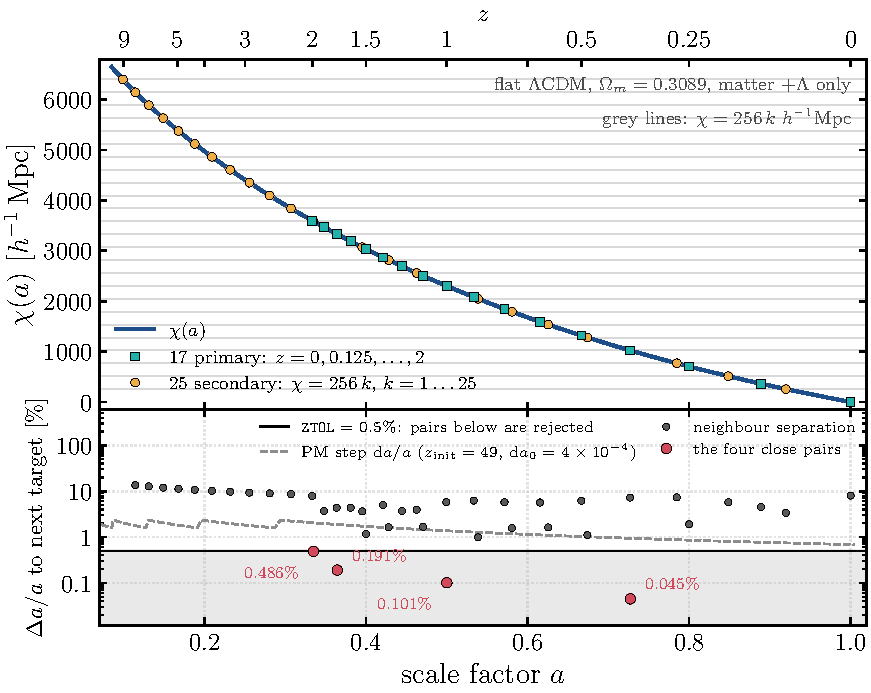
\includegraphics[width=\linewidth,height=0.52\textheight,keepaspectratio]{figs/output_schedule.pdf}
      \par\scriptsize 17 primary $z$ + 25 stations $\chi = 256\,k\Mpch$; four pairs closer than 0.5\,\% in $a$.
    \end{column}
    \hfill
    \begin{column}{0.47\textwidth}
      \begin{phasebox}{planblue}
        {\color{planblue}\bfseries Agreed with Baojiu}\par\smallskip
        \scriptsize
        No particle snapshots (200\,GB each at $2048^3$); velocities in the BDM catalogues and the subsample.
        Lens planes: 3 axes $\times$ 4 slabs of $256\Mpch$, $4096^2$ float32, 0.8\,GB per output. 42 outputs; stations recomputed per cosmology.
      \end{phasebox}
      \vspace{0.3ex}
      \begin{phasebox}[colback=plangreen!6]{plangreen}
        {\color{plangreen}\bfseries Verified}\par\smallskip
        \scriptsize
        Baojiu's 42 scale factors = flat $\Lambda$CDM, $\Omega_m = 0.3089$, matter $+\Lambda$ only, to $8\times10^{-8}$;
        the same rule generates all 96 ECOSMOG lists ($2\times10^{-7}$). I1: close pairs accepted; a $3.3\times10^{-4}$ step
        costs one PM step and $\sim 2\times10^{-6}$ in velocity.
      \end{phasebox}
      \vspace{0.3ex}
      \begin{phasebox}[colback=planpale]{plangold}
        \scriptsize
        Companion scope: L1024 $N_g$ 4096 fiducial boxes ($2048^3$) and the 96 ECOSMOG nodes (Baojiu's $1024^3$ ICs).
      \end{phasebox}
    \end{column}
  \end{columns}
  \source{plan sections 1--2; \texttt{docs/degrace\_ecosmog/}}
\end{frame}

% -----------------------------------------------------------------------------
\begin{frame}{Shared conventions for every new product}
  \footnotesize
  \begin{columns}[T,totalwidth=\textwidth]
    \begin{column}{0.48\textwidth}
      \begin{phasebox}{planblue}
        {\color{planblue}\bfseries Fourier modes (I7, I8)}\par\smallskip
        \scriptsize
        $\tilde\delta(\mathbf k) = N^{-3}\sum_x \delta(x)\,e^{-i\mathbf k\cdot\mathbf x}$, $\mathbf k = (2\pi/L)(i_x,i_y,i_z)$, $P = L^3\langle|\tilde\delta|^2\rangle$.
        One copy routine converts from FFTPACK5's layout for every dump (they are cross-correlated mode by mode).
        Store the cube $|i_x|,|i_y| \le n$, $0 \le i_z \le n$, $n = \lfloor k_c L/2\pi \rfloor$; $k = 0$ set to zero.
        Fortran \texttt{C(0:n,-n:n,-n:n)}; numpy \texttt{reshape(2n+1,2n+1,n+1)} $\to$ \texttt{[ix+n, iy+n, iz]}.
        $i_x$ is the catalogue's $x$ axis; \texttt{axis\_map} recorded. No deconvolution inside GLAM.
      \end{phasebox}
      \vspace{0.3ex}
      \begin{phasebox}{planteal}
        {\color{planteal}\bfseries Velocity epoch}\par\smallskip
        \scriptsize
        GLAM outputs are not synchronous: $x$ at $a$, $v$ at $a - \mathrm{d}a/2$ with the step just taken
        (down to $3.3\times10^{-4}$ in exact-$z$ mode). Every product with velocities uses the BDM pair and records \texttt{a\_x}, \texttt{a\_v}.
      \end{phasebox}
    \end{column}
    \hfill
    \begin{column}{0.48\textwidth}
      \begin{phasebox}{plangold}
        {\color{plangold}\bfseries Files}\par\smallskip
        \scriptsize
        Raw little-endian binary, \texttt{access='stream'}, explicit \texttt{convert='little\_endian'} (the build is big-endian), no record markers.
        Sidecar \texttt{.meta} with \texttt{key = value}: \texttt{git\_hash}, \texttt{model}, \texttt{fR0}, \texttt{L}, \texttt{N\_p}, \texttt{N\_g}, \texttt{N\_dep},
        \texttt{a}, \texttt{z}, \texttt{a\_x}, \texttt{a\_v}, \texttt{step}, \texttt{box}, \texttt{units}, \texttt{axis\_map}, \texttt{D\_code(a)}, plus item keys.
        Names: \texttt{extra/<run>\_a<a>\_<product>.\{bin,meta\}} or GLAM's \texttt{<product>.<step>.<box>.dat}: decide once.
      \end{phasebox}
      \vspace{0.3ex}
      \begin{phasebox}{plangreen}
        {\color{plangreen}\bfseries Parameters}\par\smallskip
        \scriptsize
        New flags appended to the end of \texttt{Init.dat} and mirrored in \texttt{Setup.dat} (\texttt{PMP2init}), read by \texttt{ReadSetup} with \texttt{iostat}
        and defaults off, so every existing run directory stays valid.
      \end{phasebox}
    \end{column}
  \end{columns}
  \source{plan section 3}
\end{frame}

% -----------------------------------------------------------------------------
\begin{frame}{Sequence at an output step: one deposit serves everything}
  \footnotesize
  \centering
  \begin{tikzpicture}[node distance=3mm and 3mm]
    \node[process=planblue,text width=20mm] (dens) {\texttt{DENSIT}\\CIC $\delta$ into \texttt{FI}};
    \node[process=planteal,text width=20mm,right=of dens] (lens) {I2 lens planes\\slab sums of \texttt{FI}};
    \node[process=plangold,text width=22mm,right=of lens] (fft) {P(k) FFT of \texttt{FI}\\+ I8 $\delta_m$ modes\\$|k_i| \le k_{c,\delta}$};
    \node[process=plangold,text width=22mm,right=of fft] (mom) {I8 momentum\\reuse \texttt{FI} $\times 3$\\$p_x, p_y, p_z$};
    \node[process=planrose,text width=20mm,right=of mom] (sub) {I9 subsample\\particle arrays};
    \node[process=planblue,text width=18mm,below=of mom] (bdm) {\texttt{BDM}\\re-deposits \texttt{FI}};
    \node[process=plangreen,text width=22mm,left=of bdm] (fr) {I10 $f_R$ at halo\\centres (f(R))};
    \draw[flow] (dens) -- (lens);
    \draw[flow] (lens) -- (fft);
    \draw[flow] (fft) -- (mom);
    \draw[flow] (mom) -- (sub);
    \draw[flow] (sub) |- (bdm);
    \draw[flow] (bdm) -- (fr);
  \end{tikzpicture}

  \vspace{1ex}
  \begin{columns}[T,totalwidth=\textwidth]
    \begin{column}{0.48\textwidth}
      \begin{phasebox}[colback=planpale]{planblue}
        \scriptsize
        Today \texttt{Analysis} runs PDF $\to$ P(k) (\texttt{GetPower} FFTs \texttt{FI} in place, \texttt{mDENSIT=1}) $\to$ dump/project $\to$ bias $\to$ \texttt{BDM(mDENSIT)}.
        The new products slot in without a second deposit: lens planes and the $\delta_m$ modes use the same CIC field; the momentum deposits
        reuse \texttt{FI}, which nothing reads again before \texttt{BDM} (Phase 0, Q5, to confirm).
      \end{phasebox}
    \end{column}
    \hfill
    \begin{column}{0.48\textwidth}
      \begin{phasebox}[colback=plangreen!6]{plangreen}
        \scriptsize
        \textbf{Memory:} zero extra $N_g^3$ arrays with $N_{\rm dep} = N_g$; 0.8\,GB for the planes; the mode cubes are $\le 0.5$\,GB.
        A separate $N_g/2$ buffer (34\,GB) only if \texttt{sacct} MaxRSS shows headroom (Q8).
        \texttt{MG\_scratch\_release} already frees multigrid scratch around outputs.
      \end{phasebox}
    \end{column}
  \end{columns}
  \source{plan section 4; \texttt{PMP2mod\_analyze.f90} \texttt{Analysis}, \texttt{PMP2mod\_density.f90}, \texttt{PMP2mod\_power.f90}}
\end{frame}

% -----------------------------------------------------------------------------
\begin{frame}{Track A: campaign readiness (I2--I6)}
  \footnotesize
  \begin{columns}[T,totalwidth=\textwidth]
    \begin{column}{0.48\textwidth}
      \begin{phasebox}{planteal}
        {\color{planteal}\bfseries I2 Lens planes}\par\smallskip
        \scriptsize
        Generalise \texttt{ProjectDENSIT}: per axis, mean $(1+\delta)$ of each slab column, optional block average, OpenMP as today.
        Flags \texttt{LENS\_SLABS} (4), \texttt{LENS\_GRID} (4096). One \texttt{.bin} per output, 12 planes X$_{1..4}$ Y$_{1..4}$ Z$_{1..4}$ + \texttt{.meta}.
        Logged: plane means $= 1$, slabs sum to the full projection.
      \end{phasebox}
      \vspace{0.3ex}
      \begin{phasebox}{planblue}
        {\color{planblue}\bfseries I3 Schedule input and generator}\par\smallskip
        \scriptsize
        \texttt{\#outputs = -42} + redshifts (never $z_{\rm init}$). Generator: ECOSMOG nodes from \texttt{aout.json}/\texttt{nodes.csv};
        new cosmologies from $\chi(a)$ + the 17 primary $z$; writes the \texttt{Init.dat} block and the \texttt{PkTable.dat} header.
        Reproduces the fiducial list to $10^{-7}$, all 96 lists to $10^{-6}$.
      \end{phasebox}
    \end{column}
    \hfill
    \begin{column}{0.48\textwidth}
      \begin{phasebox}{plangold}
        {\color{plangold}\bfseries I4 Index file}\par\smallskip
        \scriptsize
        \texttt{OutputSchedule.dat} at run start: \texttt{ISTEP a z chi exact class} per marked step; halocat maps snapshot numbers from it.
      \end{phasebox}
      \vspace{0.3ex}
      \begin{phasebox}{planrose}
        {\color{planrose}\bfseries I5 One per-output class list}\par\smallskip
        \scriptsize
        \texttt{iBDM}, \texttt{iPower}, lens planes and \texttt{EXTRA\_OUTPUT} must not all fire at 42 outputs.
        One class list (e.g.\ 1 = primary: BDM + P(k) + planes + extras; 2 = station: planes + P(k)) replaces the brief's
        \texttt{EXTRA\_OUTPUT\_LIST}. Default to agree with Baojiu.
      \end{phasebox}
      \vspace{0.3ex}
      \begin{phasebox}{plangreen}
        {\color{plangreen}\bfseries I6 Configuration and provenance}\par\smallskip
        \scriptsize
        \texttt{iSave=0}, \texttt{iPower=1}, \texttt{iBDM=1}, planes on, \texttt{Pk tune = 1.0}, $z_{\rm init}$ 49, $\mathrm{d}a_0$ by the rule,
        \texttt{Ncheckpoint} so a lost 72\,h job does not restart from $z_{\rm init}$. Record \texttt{Init.dat}, the index file, the \texttt{ic2pm} epoch line, \texttt{.meta} sidecars.
      \end{phasebox}
    \end{column}
  \end{columns}
  \source{plan section 5, I2--I6}
\end{frame}

% -----------------------------------------------------------------------------
\begin{frame}{Track B: extra on-the-fly outputs (I7--I11)}
  \footnotesize
  \begin{columns}[T,totalwidth=\textwidth]
    \begin{column}{0.48\textwidth}
      \begin{phasebox}[colback=planpale]{plangold}
        {\color{plangold}\bfseries Why}\par\smallskip
        \scriptsize
        Mass-pair $\xi_{hh}$ is shot-noise limited above $\log M \sim 14.5$: use halo $\times$ matter and halo $\times$ momentum
        cross-correlations instead. Store the matter side; keep mark, bin and rank definitions offline.
      \end{phasebox}
      \vspace{0.3ex}
      \begin{phasebox}{planblue}
        {\color{planblue}\bfseries I7 $\delta_L(k)$ (Item A)}\par\smallskip
        \scriptsize
        Modes $|k_i| \le 1.5$ of the initial Gaussian field, linear-theory normalised at $a = 1$ with the code's growth; identical files for
        f(R) and $\Lambda$CDM with the same seed. Gives a cosmic-variance-free halo propagator $\Gamma_h(k|M)$. Route to decide (next slide).
      \end{phasebox}
      \vspace{0.3ex}
      \begin{phasebox}{plangold}
        {\color{plangold}\bfseries I8 low-$k$ $\delta_m$ and $(1+\delta)\mathbf v$ (Item B)}\par\smallskip
        \scriptsize
        $k_{c,\delta} = 1.5$ (3.0 if $R \approx 1\Mpch$ tidal fields are needed), $k_{c,p} = 1.0$; CIC on $N_{\rm dep} = N_g$ reusing \texttt{FI}.
        Files \texttt{deltam}, \texttt{mom\_x,y,z}.
      \end{phasebox}
    \end{column}
    \hfill
    \begin{column}{0.48\textwidth}
      \begin{phasebox}{planrose}
        {\color{planrose}\bfseries I9 1\,\% quantised subsample (Item C)}\par\smallskip
        \scriptsize
        Keep particle if \texttt{splitmix64(ID xor SALT) mod 100 == 0} (C via \texttt{iso\_c\_binding}, Python twin); increasing ID order, IDs implicit.
        int16 positions (15.6\,kpc/h) and velocities (0.25\,km/s): 12\,B per particle, 1.03\,GB at $2048^3$. Baojiu's \texttt{ics.*}
        are in lattice order with sequential IDs.
      \end{phasebox}
      \vspace{0.3ex}
      \begin{phasebox}[top=0.6mm,bottom=0.6mm]{plangreen}
        {\color{plangreen}\bfseries I10 $f_R$ at halo centres (Item D)}\par\smallskip
        \scriptsize
        Not recoverable offline: \texttt{fR\_centre} (CIC at the BDM centre), \texttt{fR\_mean} (within the BDM radius); float32, catalogue order,
        after BDM while the field is in memory.
      \end{phasebox}
      \vspace{0.3ex}
      \begin{phasebox}[colback=coolgray!6,top=0.6mm,bottom=0.6mm]{coolgray}
        \scriptsize
        \textbf{I11 (fallback):} tidal ladder $T_{ij}$, $R \in \{1,2,4,8\}$, only if the I8 dump is too large.
        \textbf{Not in GLAM:} marks, binning, eigen-decomposition, Python readers.
      \end{phasebox}
    \end{column}
  \end{columns}
  \source{plan sections 5 (I7--I11) and 6}
\end{frame}

% -----------------------------------------------------------------------------
\begin{frame}{Decision: the source of $\delta_L$ under the 2LPTIC rule}
  \footnotesize
  \begin{phasebox}[colback=planred!5]{planred}
    {\color{planred}\bfseries Conflict}\par\smallskip
    \scriptsize
    The brief places the $\delta_L$ dump in \texttt{PMP2start}, but new runs never use \texttt{PMP2start}: the Gaussian field is generated by the
    FML generator (our boxes) or by Baojiu's 2LPTic (ECOSMOG companions).
  \end{phasebox}
  \vspace{0.6ex}
  \begin{columns}[T,totalwidth=\textwidth]
    \begin{column}{0.32\textwidth}
      \begin{phasebox}{plangreen}
        {\color{plangreen}\bfseries Route 1: FML generator}\par\smallskip
        \scriptsize
        Add the dump to \texttt{2LPTIC\_Gui/} (our code): same copy convention and file format. Covers every new box.
        Cleanest; needs the generator's RNG and ordering recorded (Phase 0, Q1--Q2).
      \end{phasebox}
    \end{column}
    \hfill
    \begin{column}{0.32\textwidth}
      \begin{phasebox}{plangold}
        {\color{plangold}\bfseries Route 2: Baojiu's \texttt{ics.*}}\par\smallskip
        \scriptsize
        (a) derive $\delta_L = -\nabla\!\cdot\!\Psi$ from the IC displacements at ingest in \texttt{ic2pm}; the 2LPT term contaminates at the
        per-cent level near $k \sim 1$, negligible at $k < 0.1$ (quantify with V3); or (b) patch his 2LPTic for a regenerate-only dump with
        his \texttt{2LPTic.param} and seed 2026 (code and parameters on cosma7).
      \end{phasebox}
    \end{column}
    \hfill
    \begin{column}{0.32\textwidth}
      \begin{phasebox}{planblue}
        {\color{planblue}\bfseries Route 3: legacy pilots}\par\smallskip
        \scriptsize
        The brief's \texttt{IC\_DUMP\_ONLY} mode in \texttt{PMP2start} for the existing ZA-at-$z{=}100$ pilots: generate the field with the
        pilot's parameters and seed, write, exit. Needs the RNG thread-dependence answer.
      \end{phasebox}
    \end{column}
  \end{columns}
  \vspace{0.6ex}
  \begin{phasebox}[colback=planpale]{plangold}
    \scriptsize
    Proposal: route 1 for new boxes and route 2(a) for the ECOSMOG companions, validated against 2(b) on one node; route 3 only if $\Gamma_h$ for the
    legacy pilots is still wanted. All three write the same \texttt{deltaL.\{bin,meta\}} and pass V1, V7, V8.
  \end{phasebox}
  \source{plan section 5, I7}
\end{frame}

% -----------------------------------------------------------------------------
\begin{frame}{Validation and storage}
  \footnotesize
  \begin{columns}[T,totalwidth=\textwidth]
    \begin{column}{0.53\textwidth}
      \scriptsize
      \setlength{\tabcolsep}{3pt}
      \begin{tabular}{@{}l>{\raggedright\arraybackslash}p{0.66\linewidth}@{}}
        \toprule
        test & pass criterion \\
        \midrule
        S1--S2 schedule & 65/65; generator to $10^{-7}$ / $10^{-6}$ \\
        L1--L3 planes & means $=1$; equals the offline projection; plane $P(k)$ vs 3-D $P(k)$ \\
        V1 layout & $\cos/\sin$ modes at $\pm m$, amplitude 1/2 \\
        V2 $P(k)$ & \texttt{deltam} vs code $P_{mm}$ within $10^{-3}$ \\
        V3 closure & \texttt{deltam}($a_{\rm ini}$)/\texttt{deltaL} $= D_{\rm code}$ to 0.5\,\%, $r > 0.999$ \\
        V4 halo axes & $r \gtrsim 0.9$ at low $k$, no linear-in-$k$ phase \\
        V5 subsample & $n_{\rm sel}$ within $3\sigma$; IDs, positions match; hashes agree \\
        V6 momentum & subsample vs \texttt{mom\_*} within shot noise \\
        V7--V8 determinism & identical md5 (threads; f(R) vs $\Lambda$CDM) \\
        V9 overhead & $< 5\,\%$ wall time; RSS within node memory \\
        \bottomrule
      \end{tabular}
    \end{column}
    \hfill
    \begin{column}{0.44\textwidth}
      \scriptsize
      \setlength{\tabcolsep}{3pt}
      \begin{tabular}{@{}lrr@{}}
        \toprule
        per output & $2048^3$ & $1024^3$ \\
        \midrule
        lens planes $12\times4096^2$ & 0.8\,GB & 0.8\,GB \\
        \texttt{CatshortV} & 0.3--0.4\,GB & $\sim$0.1\,GB \\
        \texttt{deltam} ($k_c$ 1.5 / 3.0) & 0.47 / 3.7\,GB & same \\
        \texttt{mom\_x,y,z} ($k_c$ 1.0) & 0.41\,GB & same \\
        subsample $M = 100$ & 1.03\,GB & 0.13\,GB \\
        \texttt{deltaL} (once per run) & 0.47\,GB & same \\
        \bottomrule
      \end{tabular}
      \vspace{0.6ex}
      \begin{phasebox}[colback=planred!5]{planred}
        {\color{planred}\bfseries Budget decision}\par\smallskip
        \scriptsize
        Per $2048^3$ box: planes 34\,GB, catalogues $\sim$15\,GB, extras at all 42 outputs $\sim$80\,GB
        ($\approx$130\,GB per box, 13\,TB for 100 boxes); extras at the 17 primary outputs only $\sim$32\,GB ($\approx$80\,GB, 8\,TB).
        Baojiu's 3.4\,TB covered lens planes alone.
      \end{phasebox}
    \end{column}
  \end{columns}
  \source{plan sections 8--9}
\end{frame}

% -----------------------------------------------------------------------------
\begin{frame}{Phasing and open questions}
  \footnotesize
  \begin{columns}[T,totalwidth=\textwidth]
    \begin{column}{0.46\textwidth}
      \begin{phasebox}{planblue}
        {\color{planblue}\bfseries Order of work} (each phase: code, numbers, section-16 entry)\par\smallskip
        \scriptsize
        \begin{enumerate}\setlength\itemsep{0.2em}
          \item Phase 0 reconnaissance (plan section 13), no edits; report.
          \item I3 generator + S2; I4 index; I5 class list.
          \item I2 lens planes + L1--L3.
          \item Pilot ECOSMOG node 2: ingest, run $\Lambda$CDM + f(R), compare $P(k)$ with the twins; runtime, \texttt{sacct}, sizes.
          \item I7 (route decided) + V1, V7, V8; $\delta_L$ for one legacy pilot + V4.
          \item I8 + V2--V4; \;7. I9 + V5--V6; \;8. I10 on the f(R) test box.
          \setcounter{enumi}{8}
          \item V9 production-size overhead run, after approval.
        \end{enumerate}
      \end{phasebox}
    \end{column}
    \hfill
    \begin{column}{0.52\textwidth}
      \begin{phasebox}[colback=planpale]{plangold}
        {\color{plangold}\bfseries For Baojiu}\par\smallskip
        \scriptsize
        BDM at all 42 or the 17 primary? Lens planes at primary epochs too? Plane normalisation (mean $1+\delta$ vs surface density)?
        Keep both members of close pairs? Plus the ECOSMOG questions (CAMB $\omega_c$, r2g conversions, Node\_900, $\Lambda$CDM $P(k)$).
      \end{phasebox}
      \vspace{0.3ex}
      \begin{phasebox}[colback=planpale]{planrose}
        {\color{planrose}\bfseries For CZ}\par\smallskip
        \scriptsize
        Extras cadence (all 42 vs primary only); $k_{c,\delta}$ 1.5 or 3.0; the $\delta_L$ route; file naming scheme;
        companion resolution ($N_g$ 2048 or 4096 on $1024^3$ particles); confirm the track order above.
      \end{phasebox}
      \vspace{0.3ex}
      \begin{phasebox}[colback=plangreen!6]{plangreen}
        \scriptsize
        Phase-0 facts already recorded in section 16: lattice order of Baojiu's ICs; $v$ at $a - \mathrm{d}a/2$ at outputs;
        \texttt{FI} life cycle in \texttt{Analysis}; \texttt{FI2}/\texttt{FI3} for MG; 950+\,GB for f(R) at $N_g$ 4096; sequential \texttt{Init.dat} parser.
      \end{phasebox}
    \end{column}
  \end{columns}
  \source{plan sections 10, 11, 13, 16}
\end{frame}

\end{document}
